\chapter{Casi d'Uso}

\todo{rivedere la numerazione dei casi d'uso}

\section{UC1}

\section{UC2}

\section{UC3 - Accesso al Manuale Utente}

\begin{figure}[h]
  \centering
  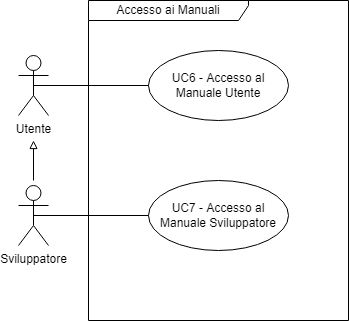
\includegraphics[width=0.6\textwidth]{UC_manuali}
  \caption{UC3 UC4 - Accesso ai manuali utente e sviluppatore}
\end{figure}

\begin{itemize}
  \item \textbf{Descrizione}: l'utente che ha un dubbio o vuole più informazioni sull'utilizzo dell'applicazione, deve avere accesso rapido al manuale utente;
  \item \textbf{Attore primario}: utente;
  \item \textbf{Precondizioni}: nessuna, l'opzione di accesso ai manuali deve essere sempre disponibile all'utente;
  \item \textbf{Postcondizioni}: viene visualizzato il manuale utente;
  \item \textbf{Scenario principale}: 
  \begin{enumerate}
    \item L'utente seleziona il "manuale utente";
    \item Viene visualizzato il manuale utente.
  \end{enumerate}
\end{itemize}

\section{UC3 + 1 - Accesso al Manuale Sviluppatore}

\begin{itemize}
  \item \textbf{Descrizione}: essendo Login Warrior un progetto open source, un qualsiasi utente deve avere accesso ad un manuale sviluppatore (sia per manutenere, sia per estendere il software);
  \item \textbf{Attore primario}: utente;
  \item \textbf{Precondizioni}: nessuna, l'opzione di accesso ai manuali deve essere sempre disponibile all'utente;
  \item \textbf{Postcondizioni}: viene visualizzato il manuale sviluppatore;
  \item \textbf{Scenario principale}: 
  \begin{enumerate}
    \item L'utente seleziona il "manuale sviluppatore";
    \item Viene visualizzato il manuale sviluppatore.
  \end{enumerate}
\end{itemize}

\section{UC4}

\section{UC5}

\section{UC6}

\section{UC7}